\chapter{Generating Art with Computers}
\label{ch:art-computers}

This book has explored deep connections between logic
and computing, including the use of equations and logic to
write and analyze computer programs. In this chapter we're going
to turn our attention to artistic creativity. Can logic and
equations be useful in creating works of art?

\section{Representing Images in a Computer}

To create visual art with a computer, we need some way to
represent images in computers. How does a computer
store a picture?
The answer, it turns out, is surprisingly pedestrian. Ignoring
color for now, you can think of a computer display, such as the
screen on your computer or phone, as a collection of millions
of tiny dots arranged in a rectangular \index{grid, image}grid with a fixed number
of rows and columns. Different displays have different dimensions.
For reference, let's say there are $M$ rows and $N$ columns
in the grid.
Each dot is called a \index{pixel}\emph{pixel}, a term in common use now
that at one time was short for \index{picture}``picture element.''

The computer we are using right now has
a $1440\times900$ display: 900 rows and 1440 columns.
Continuing to ignore color for the moment, each pixel can
be either emitting light (turned on) or not emitting light
(turned off), so a picture in a computer can be represented
by specifying which pixels are ``on'' and which
are ``off.'' A straightforward way to do this is to use a list of
numbers in which each number corresponds to a pixel. Even better,
we can use a list of rows, each of which is list of $N$
0/1 elements (one for each pixel in the row).
The off/on status of the pixels in the row would
match the 0/1 elements in the list,
and there would be $M$ such lists, one for each row on the display.
This list of lists forms a kind of \index{matrix}matrix.

Figure~\ref{fig:glider-in-images} illustrates
this idea with a $4\times4$ grid of squares
representing a $4\times4$ section of pixels in a computer display.
The pixel in row $i$ and column $j$ is ``on''
(indicated in the figure by a black square in the diagram)
when the $j^\text{th}$
entry in the $i^\text{th}$ list is a 1.
When the entry is a 0, the pixel is ``off'' (indicate by white square).

\begin{figure}
\begin{center}
\begin{minipage}{3cm}
\begin{verbatim}
 [[0 1 0 0]
  [0 0 1 0]
  [1 1 1 0]
  [0 0 0 0]]
\end{verbatim}
\end{minipage}%
\begin{minipage}{3cm}
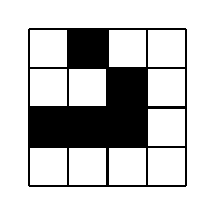
\begin{tikzpicture}[thick, scale=0.5]
\draw (0,0) grid (4,4);
\foreach \c in {(0,1), (1,1), (2,1), (2,2), (1,3)}
    \fill \c + (1, 1) rectangle \c;
\end{tikzpicture}
\end{minipage}
\end{center}
\caption{A Picture Encoded as a Matrix of Pixels}
\label{fig:glider-in-images}
\end{figure}

Using lists to represent \index{image}images is an important concept.
The first chapter of the book talked about boundaries
and interfaces between software and hardware, and these ideas are
well illustrated in this representation of images.
Lists are a well-studied notion and have played a central
role throughout the book.
You probably have a solid grasp of lists at this point.
Now we are using them to represent pictures, which are
physical entities in the real world.
From the software perspective,
generating an image amounts to generating a list of numbers.
It is up to the hardware to interpret the list of numbers
as an image and display it.
We have used equations to generate lists in many contexts,
and these ideas are directly applicable in this new context.

This kind of \index{layering}layering is a common strategy for dealing
with complex problems in computer science.
Each layer in the solution provides a service
to the layers next to it. In this example,
the software layer generates lists of zeros and ones
for the hardware layer, and
the hardware layer turns lists of zeros and ones into physical images.
Both layers represent images, but in different forms.
The software generates an abstraction of an image
in the form of zeros and ones,
and the hardware layer turns that abstraction into an
image on a screen. That is, the hardware builds a
concrete version of the abstraction specified by software.
So far in this example there are only two layers,
but in complex systems, there can be dozens of layers.

So far, so good, with \index{black-and-white}\index{image!black-and-white}black-and-white images,
but what about \index{color}color \index{image!color}images?
The \index{eye, human}human eye perceives
color using specialized cells, called \emph{cones}, in the central
part of the retina. There are three types of cones, each one sensitive
to a different range of colors. There is some overlap in the range
of colors that each type of cone can detect, but it is mostly accurate
to think in terms of cones that are sensitive to shades of red, green,
and blue.

So, color images can be created by using three dots on a screen
for each \index{pixel!color}\index{color!pixel}pixel,
one for red, one for green, and one for blue.
If the red dot in a pixel is on, and the green and blue dots
are off, the pixel looks red. Other colors come from combinations
of red, green, and blue dots.
The following list represents the first row of pixels
in the black-and-white image shown in
Figure \ref{fig:glider-in-images}.
\begin{quote}
    \textsf{[0 1 0 0]}
\end{quote}
In a color image, the row of pixels could be represented by
a list of three-element lists.
\begin{quote}
    \textsf{[[0 0 0] [1 0 0] [0 0 0] [0 0 0]]}
\end{quote}
In this representation, colors are specified as triples of 0/1 values
specifying the off/on status of the color dots in the corresponding pixel.
The first element of the triple is for the red dot, the second
for the green dot, the third for the blue dot.
That is the conventional order:
\index{red-green-blue }red-green-blue (\index{RGB}RGB).
In this scheme, \textsf{[1 0 0]} represents pure red,
so the list, as shown, represents a red dot in the second pixel of the row.

With this convention, there would be eight possible \index{color!eight}colors because
each element in the triple can be either zero or one,
which leads to $2^3$ (that is, $8$) combinations:
black \textsf{[0 0 0]},
white \textsf{[1 1 1]},
red \textsf{[1 0 0]},
green \textsf{[0 1 0]},
blue \textsf{[0 0 1]},
cyan \textsf{[0 1 1]},
magenta \textsf{[1 0 1]},
and
yellow \textsf{[1 1 0]}.
That might be an improvement over black-and-white,
but it's a crude representation of color
compared to the colors the eye can perceive.

Getting more colors requires a more subtle blending of
red, green, and blue. For example, a pixel with red and green
on and blue off will appear to be yellow,
but by using a range of \index{color!intensity}color intensities,
not just on and off, a blend of red and green can produce other
colors, such as orange. The human eye can detect more than 256 shades of
each color, but 256 shades are enough to produce realistic color.
So, it is common to represent color intensity as a number
from 0 to 255. Using this scheme, the list \textsf{[255 140 0]} produces
a dark shade of \index{orange}orange.

In principle, a matrix of \index{red-green-blue}red-green-blue
intensities is
enough to create images, even colorful images.
However, additional layers between the software and hardware
layers can be helpful. Imagine, for example, an operator called \textsf{line}
that paints a line on an image. This operator would figure out
which pixels are on the line and build a matrix with
the appropriate triple for the chosen color at each of those pixels.
\begin{quote}
    \textsf{(line} $image$ $x_1$ $y_1$ $x_2$ $y_2$ $color$\textsf{)}
\end{quote}
The $image$ operand is a matrix of pixels (red-green-blue triples)
representing an image, the $x$ and $y$ values
specify the row/column coordinates of the endpoints of the line,
and $color$ is a triple of red-green-blue color intensities.
The operator delivers a new matrix of color intensities
like the $image$ operand, but with the specified color
at each pixel on the line.

\begin{aside}
Drawing a \index{line!draw}line from one point to another on a grid of points is tricky.
There are many subtle cases to consider, and
if you don't make good choices, the result does not look
like a line at all. If the starting point has
coordinates $(1,1)$ and the end point $(10,10)$,
then the line consists of the points $(1,1)$,
$(2,2)$, $(3,3)$, and so on up to $(10,10)$.
No problem.

However, if the end point is $(2,10)$ instead of $(10,10)$,
then choosing the right points for the line is more difficult.
Sketch a $10\times10$ grid and try drawing a \index{image!line}line
from  $(1,1)$ to  $(2,10)$.
This is an extreme case, but many lines lead to similar issues.
Geometry on a grid,
\index{digital geometry}\index{geometry, digital}digital geometry,
presents a lot of problems like this one that are hard to solve.

Another problem is speed. In many graphics applications, the
computer needs to draw millions or billions of lines per second,
so speed is important.
In the 1960s, the computer scientist
\index{Bresenham, Jack}Jack Bresenham invented
a fast way to compute the list of grid points closest to the line
between any two given endpoints.
Most of the line-drawing in digital images, still today,
makes use of some version of the Bresenham algorithm.
\caption{Bresenham Line-Drawing Algorithm}
\label{aside:Bresenham}
\end{aside}

We're sure you can think of many other useful operators in
the same vein as the operator \textsf{line}. Operators to draw
triangles, squares, rectangles, polygons, circles,
ellipses, and the like. The important thing to realize is that all of
these operators work on an image represented as a matrix of
color intensities.
The operators add to the system a layer that understands
basic geometric shapes on top of the layer that represents an image
as a matrix of pixels.

Operators that create shapes are not the whole story.
Operators of another kind blur \index{image!blur}images in useful ways.
For example, suppose that an image has a
very dark line on a bright background. This creates a
sharp boundary between the line and the background, but it can be
smoothed out by averaging the colors of neighboring pixels.
The bright pixels on one side of the boundary become a little darker,
and the dark pixels on the other side become a little lighter,
resulting in a more subtle boundary. This is the basic idea behind
operators that manipulate images at the level
of individual pixels and their neighbors. Image-processing operators
of this kind form a class of  known as \index{filter}\emph{image filters}.
There are a lot of filters in image
processing software, and they provide another abstraction layer
that facilitates creating representations of images with software.

\section{Generating Images Randomly}

One way to generate artistic images is to insert a layer of
randomness on top of the layers that create geometric shapes.
An artist may layer \index{painting}paints on a canvas
with a brush that has a certain texture, and the brush strokes
will create a complex pattern that is more than just a line.
Figure~\ref{fig:line-art} shows a pair of images.
One is a straight line
and the other shows how adding a lot of nearby, short lines in
more-or-less random orientations
creates an image similar to a line, but with more texture,
like a brush stroke, perhaps.
Similar operations can produce
other geometric shapes with a degree of randomness,
such as in noisy rectangles or circles that are
mostly, but not exactly, round.

\begin{figure}
\begin{center}
\begin{tabular}{ll}
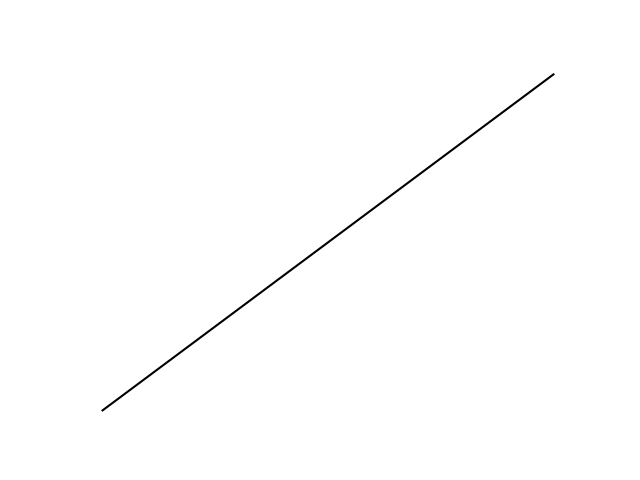
\includegraphics[scale=0.3]{images/straight-line.png} &
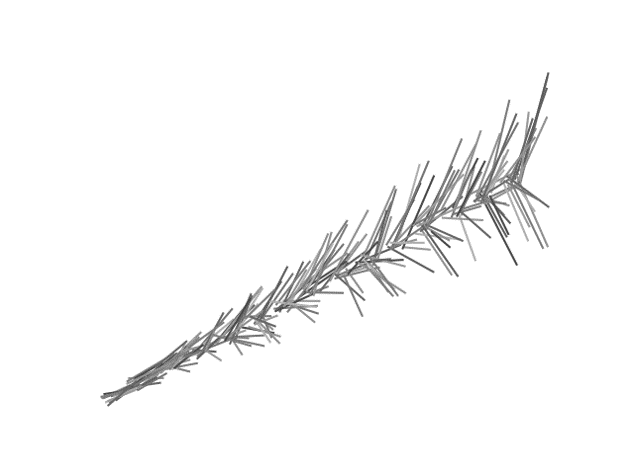
\includegraphics[scale=0.3]{images/random-line-art.png} \\
\end{tabular}
\end{center}
\caption{Straight Line vs.~a Line Made Up of Random Segments}
\label{fig:line-art}
\end{figure}

But what do we mean by \index{random}random?
None of the digital circuits
that we have studied exhibit random behavior.
Instead, they conform to precise equations and deliver the same
results every time they are supplied with the same data.
The following sequence of numbers appears to be random.
$$0, 1, 5, 3, 4, 8, 6, 7, 2, 0$$
However, it is not random. It is produced by an
operator $r$ defined by the following equations,
which are presented in both traditional, algebraic form
and in ACL2 notation.\footnote{You can ignore the ACL2
if you have not yet studied the chapters that introduce it.
The ACL2 versions of the equations don't add any information
necessary to understanding the concepts presented in this chapter.}

\begin{center}
\begin{tabular}{ll}
$r(n+1) = (4\cdot r(n) + 1)$ $mod$ $9$ & \{r1\}\\
$r(0) = 0$                        & \{r0\}\\
\end{tabular}
\end{center}

\begin{Verbatim}
(defun r (n)
 (if (zp n)
     0                                 ; {r0}
     (mod (+ (* 4 (r (- n 1))) 1) 9))) ; {r1}
\end{Verbatim}

As you can easily check if you
recall that ($x$ $mod$ $d$) is the remainder in
the division $x \div d$
(Aside~\ref{third-grade-division}, page \pageref{third-grade-division}),
$r(0) = 0$, $r(1) = 1$, $r(2
) = 5$, $r(3) = 3$,
and so on.
So, $r$ is an operator that appears to produce random
numbers, but the process is completely deterministic.
The sequences produced by such operators
are called \emph{pseudo-random}
\index{random!pseudo}\index{pseudo-random}\index{sequence!pseudo-random}sequences,
and they provide a way to introduce an aspect of randomness into images.

There are many ways to produce pseudo-random sequences.
It is a well-studied problem with a long history and lots
fascinating ramifications. It happens that the operator
$r$ belongs to the most commonly used
family of pseudo-random number generators: the
\index{random!number generator}\index{linear congruential}linear congruential generators.
A linear congruential generator has a \emph{seed}, which is
the value it delivers as the first number in the sequence.
It also has a \emph{multiplier}, an \emph{increment}, and a \emph{modulus}.
The $(n+1)^\text{th}$ number in the sequence
is produced by multiplying the $n^\text{th}$ number by
the multiplier, adding the increment, and delivering
the remainder when that sum is divided by the modulus.
The multiplier, increment, and modulus for the operator $r$
are $4$, $1$, and $9$, respectively.
One of the effects of the modulus is to keep the numbers
within a certain range, which is the range $0$, $1$, \dots $8$ in
the case of the operator $r$.

It is common to define pseudo-random operators like $r$ in
manner that, to compute a number in the pseudo-random sequence,
requires the previous value in the sequence as the operand.
This is different from the definition of $r$, where the
operand is the index of the number in the sequence: $r(n)$ is the
$n^\text{th}$ number in the sequence.
It turns out that more common method,
in which each invocation
supplies the value delivered by the previous invocation as
the operand, is much faster than
the operator $r$
because the definition is no longer inductive,
as shown in the following definition of the operator
$rs$.\footnote{Again, you won't miss the point
if you ignore the ACL2 version of the equations.}

\begin{center}
\begin{tabular}{ll}
$rs(s) = (4s + 1)$ $mod$ $9$ & \{rs\}\\
\end{tabular}
\end{center}

\begin{Verbatim}
(defun rs (s)
  (mod (+ (* 4 s) 1) 9))  ; {rs}
\end{Verbatim}

Because the modulus is 9 in the definitions of the operators
$r$ and $rs$, they always deliver a natural number between 0 and 8.
All linear congruential random number generators
have a fixed range (although it is usually a much bigger range than 0 to 8),
so they always deliver
a natural number between 0 and $D-1$, where $D$ is the modulus.\footnote{It
is often more convenient to work with random numbers between $0$ and $1$
instead of integers between zero and the modulus.
That is easily accomplished by dividing the generated number
by the modulus.}

\begin{figure}
\begin{center}
\begin{tabular}{lll}
$ragged(image, x_1, y_1, x_2, y_2, seed) =$  &&\{rg1\}\\
\hspace*{8mm}$ragged(line(image, x_1, y_1, rx, ry, black), x, y, x_2, y_2, s)$ & if $x_1 < x_2$ &\\
\hspace*{4mm}where &&\\
\hspace*{4mm}$s = rs(seed)$    &&\\
\hspace*{4mm}$jostle = s/9 - 1/2$    &&\\
\hspace*{4mm}$slope = (y_2 - y_1)/(x_2 - x_1)$    &&\\
\hspace*{4mm}$rx = x_1 + 10$     &&\\
\hspace*{4mm}$ry = y_1 + round(10\cdot(slope + jostle))$ &&\\
\hspace*{4mm}$x = x_1 + 1$     &&\\
\hspace*{4mm}$y = y_1 + round(slope)$ &&\\
\hspace*{4mm}$b =$ \textsf{[0 0 0]} &&\\
$ragged(image, x_1, x_2, y_1, y_2, seed) = image$ & if $x_1 \geq x_2$ &\{rg0\}\\
\end{tabular}

\begin{Verbatim}
(defun ragged (image x1 y1 x2 y2 seed)
 (if (< x1 x2)
     (let* ((s (rs seed))
            (jostle (- (/ s 9) 1/2))
            (slope (/ (- y2 y2) (- x2 x1)))
            (rx (+ x1 10))
            (ry (+ y1 (round(* 10 (+ slope jostle)))))
            (x (+ x1 1))
            (y (+ y1 (round slope)))
            (black (list 0 0 0)))
       (ragged (line image x1 y1 rx ry black) x y x2 y2 s) ; {rg1}
     image))                                               ; {rg0}
\end{Verbatim}
\end{center}
\caption{Operator to Draw a Ragged Line Using Random Numbers}
\label{fig:ragged-defun}
\end{figure}

The operator defined by the equations in
Figure~\ref{fig:ragged-defun} (page \pageref{fig:ragged-defun})
draws a \index{ragged line}ragged \index{line!ragged}line
by drawing short line segments at randomized angles
from starting points along the line from $(x_1,y_1)$ to $(x_2,y_2)$.
The starting points of the short line segments are
spaced one unit apart in the $x$ direction.
The $x$ coordinate of the endpoint of a short segment
is ten more than $x$ coordinate of the starting point
(that is, $x_1 + 10$).
The $y$ coordinate of that endpoint is computed
by moving in the general direction of the target
$(x_2,y_2)$, but with the direction 
randomly adjusted by a small amount.
The adjustment is made by adding a random number between
$-1/2$ and $1/2$ to the \emph{slope},
$(y_2 - y_1)/(x_2 - x_1)$, then multiplying that
number by ten (the difference between the
starting $x$ coordinates of the endpoint
and starting point of the short segment,
in the usual manner of computing coordinates
along a straight line, algebraically).

The slope used in the computation is a ratio of
two integers, but (usually) is not an integer.
Since grid-points have integer coordinates,
the numbers computed using the slope
are rounded to the nearest integer by
an operator called \textsf{round}. That way,
all of the coordinates supplied as 
operands to the \textsf{line} operator
and the operator \textsf{ragged} are pairs of
integers representing grid points.
The \textsf{line} operator won't draw any lines
that extend outside the boundaries of
the image, so if any of the computed 
coordinates are out of range, 
the line segments that are drawn will
be truncated at the image boundary.

The short segments are drawn in this way along
the line between $(x_1,y_1)$ and $(x_2,y_2)$,
with starting points whose $x$ coordinates
take all the integer values between $x_1$ and $x_2$.
This makes the starting points close together along
the points on the grid that are closest to the
line between $(x_1,y_1)$ and $(x_2,y_2)$.
The effect is a ragged line that looks more organic 
than a simple, straight line.
This is the idea behind the line
in Figure~\ref{fig:line-art} (page \pageref{fig:line-art}).

In the inductive equation \{rg1\} in the definition of the operator \textsf{ragged},
the \emph{seed} operand is supplied to the pseudo-random
number generator $rs$, and that operator uses it to produce
a number $s$ between 0 and 8. That number is supplied as the last
operand in the invocation of \textsf{ragged} in the inductive equation \{rg1\}
(so it can be used to generate the next random number),
and it is also used to \index{jostle}jostle 
the slope of the short line segment drawn by the operator \textsf{line}.
The operator \textsf{line} produces a new image,
which is the first operand in the invocation of \textsf{ragged} in equation \{rg1\}.
In this way, the image accumulates the line segments that the operator \textsf{line}
draws at each stage.

\section{Generating Purposeful Images}

Random images can be nice to look at, but should they be called art?
Can a computer program produce real works of art?
That is a philosophical question with lots of answers.
But, regardless of how you might answer the question,
there are a handful of programs that, it has been reasonably argued,
are artists. Let's look at one of them.

The program \index{AARON software}AARON,
written over a span of decades by artist \index{Cohen, Harold}Harold Cohen,
was designed in part as an exploration of artmaking. Cohen's
initial goal was to determine when a group of abstract marks can
be recognized as a coherent image. The earliest versions of his program
could do very little, and those early versions knew very little about art.
Those versions knew the difference between a figure and the ground, and also
the difference between an open figure and a closed figure, but
not much more.

What made the early versions of AARON effective was a layer that
stood on top of the low-level drawing layer. This layer was essentially
a list, but instead of pixel colors, this list contained graphical objects
and their locations. Adding a new figure to the canvas was accomplished
by adding a new object to the master list. The real breakthrough was
that this list could be examined during the process of adding
a new figure, so AARON could effectively reflect on the work it had
done earlier, then proceed with additional work.
This allowed the software to make decisions based on
artistic principles, such as balance and proportion.
This breakthrough proved so successful
that it carried over into all subsequent versions of AARON.

An obvious way to enhance AARON would have been to add more graphical
primitives, such as new figures that it could draw. But
the next step in AARON's evolution was something more profound. What
Cohen did was to enhance the program so that it could ``scribble'' around
``core figures.'' This idea came from observing the way children
scribble on paper, and in particular the key moment when the children
seemed to realize that a figure they scribbled actually represented a
realistic object in some sense. From AARON's perspective, the main improvement
was a two-step strategy where \index{core figures}core figures
were placed in a virtual world,
and then the picture was allowed to evolve by tracing a kind of path
around the core figures.
This strategy resulted in paintings with much more complexity
and a sense of realism, in that the end product showed realistic-looking
objects that seemed to be inspired by the real world. Certainly, if a
human artist had drawn these shapes, they would have been considered to be
reflections of the real world.

From this point on, AARON became more and more \emph{representational} in
the works it produced. This came from three main sources of improvement. The first
was a database of core figures that combined to represent visually some
objects from the real world. Each core figure was represented as a list of
key points that provided essentially an outline, and the figures were connected
in space and orientation.
For example, a plant could be represented by
a trunk, some branches, and some leaves. Each of those may be a core figure,
and the figures would be related to each other geometrically, which is to say
that the branches are connected to the trunk, and the leaves to the branches.
This basic strategy worked to model even complex objects, such as a basic human
form and a recognizable image of the Statue of Liberty.

The second improvement was a series of algorithms that could create reasonable
objects made up of core figures. It is not feasible to model all possible
objects using core figures. So, Cohen wrote some algorithms that allowed AARON to
imagine \index{quasi-plants}\index{plants, quasi}plants,
or as he called them \emph{quasi-plants}. It probably won't surprise
you to learn that these algorithms made extensive use of pseudo-random numbers.
At this point, AARON's paintings featured recognizable human shapes
in an environment that included many plant-like shapes.

Finally, the third improvement was the development of a set of rules that
let AARON render an image from a world described by core figures. Essentially,
these rules amount to expertise in drawing. For example, the core figures occupy
a space in three dimensions, and the rules determine how AARON is to deal with
geometric problems such as perspective and occlusion. That is, figures farther
away must appear smaller in the final image, and a core figure near the front may
partially hide a figure that is farther away. AARON is truly becoming an expert
painter, which is one aspect of being an artist.

AARON's paintings from this time represent a high point in its work, and they
have been exhibited in museums.
Nevertheless, there was a hidden limitation, in that the core figures
used to build AARON's model of the world were two-dimensional. The figures could be
placed in a three-dimensional world, but the realism in AARON's work was partially
due to the limitations in the scale of its paintings. Cohen wanted to create larger
and more complex paintings, and he felt that this increase in scale would require a
more detailed model of the real world in AARON's data structures.

So, Cohen embarked on a new modeling phase with more detailed and fully
three-dimensional models of the objects that AARON would draw, such as the human
body. These models were made of groups of three-dimensional points that were
related to other similar groups, in a way that is clearly derived from the earlier
core figures. In a tradition dating back to da Vinci and Michelangelo, the models
for the human body were taken directly from anatomical studies. This shift
created many complications because AARON's model was now three-dimensional,
so it had to create two-dimensional projections of core images before rendering a
painting.

The complications are significant, and you might find it interesting to pursue
it further by reading Cohen's own description
of his work or \index{McCorduck, Pamela}Pamela McCorduck's
very readable account of AARON's evolution as an
artist---even to the point of mixing its own pigments and painting its own artworks
on a physical canvas.

What we want to leave you with is an appreciation that
simple principles can indeed lead to complex behavior.
AARON's knowledge of the real world is encoded as a set of points,
and its expertise in drawing is encoded as a set of rules.
This is analogous to the way we used equations and logic to write programs,
create models of digital circuits, and reason about properties of those abstractions.
AARON is an impressive program, and it can be plausibly argued that it exhibits
artistic creativity. But at its core, it is
composed of simple principles that, taken as a whole, capture a way of painting.

%%% Local Variables:
%%% mode: latex
%%% TeX-master: "book"
%%% End:
